\documentclass[../manifest.tex]{subfiles}


% - describe your solution idiom, analyze it according to the framework of the book, and justify your design choices with respect to alternative possibilities
% - if you have done any significant algorithmic work, discuss the algorithm and data structures
% - you might choose to split out Interface into its own section

\begin{document}

In this section we describe our visualization solution and analyze it using the What-Why-How framework provided by \cite{Munzner:2014} for which table~\ref{tab:analysis} provides a summary.

\begin{table}
  \caption{What-Why-How analysis of Teamline.}
  \label{tab:analysis}
  \begin{tabularx}{\columnwidth}{ l | X }
    \hline
    What: Data & Table of graded commits with attributes described in \ref{tab:attributes}. \\
    \hline
    What: Derived & Measure of contribution to pass rate and coverage; contribution uniformity. These are discussed in section \ref{ssec:data-description}. \\
    \hline
    Why: Tasks & Present the uniformity of contributions and summarize the team's commit history. \\
    \hline
    How: Encode & We used a heatmap with sparklines in the overview  and line charts in the detail view. Marks are positioned on a common time scale with color indicating the attribute that is being encoded.\\
    \hline
    How: Facet & Overview + detail views. Detail view is partitioned into side-by-side views. \\
    \hline
    How: Embed & Superimpose sparklines on the overview's heatmap cells. \\
    \hline
    How: Reduce & Filtering is done by selecting the team and the deliverable. \\
    \hline
  \end{tabularx}
\end{table}

Teamline is split into two views: an \textbf{overview} providing a summary for all teams and a \textbf{team view} providing details for a given team (\textit{how: facet}). The data for both views is based on the currently selected deliverable which is controlled by buttons in the menu bar (\textit{how: reduce}).

The user is first presented the \textbf{overview} shown in figure~\ref{fig:sample-overview}\footnote{The highlighted cell is used in section~\ref{Results} and can be ignored for now.} which shows a heatmap of teams (\textit{How: Encode}) enriched with a sparkline in each cell (\textit{How: Embed}). The major attribute we want to show is the \textit{Within-team contribution uniformity} (see section~\ref{sec:abstractions}) which is encoded by saturation of the team cells: low saturation indicates uneven contribution and high saturation indicates even distribution. We chose a color-coding ranging from white (for most even contribution) to dark orange (for most uneven contribution). We discussed an alternative approach ranging from white for most uneven contribution to green for most even contribution (white = negative), but argued that TAs really aim to see at a glance what teams had uneven contribution and that a positive white and negative orange would highlight this aim better. We initially used a red color for uneven contribution but considered the appearance of the overview having a too negative overall connotation and switched to a 'warmer' orange color. The second attribute we were interested in for the overview of all teams was the \textit{progression of each team's grade}. We decided for a sparkline for each team that clearly indicates both the team's final grade and how the grade developed throughout the duration of the deliverable. The color of the sparklines matches the color of the grade line in the team view (see next paragraph). Clicking on a team cell switches to the team view of the target team.

\begin{figure}[h]
  \centering
  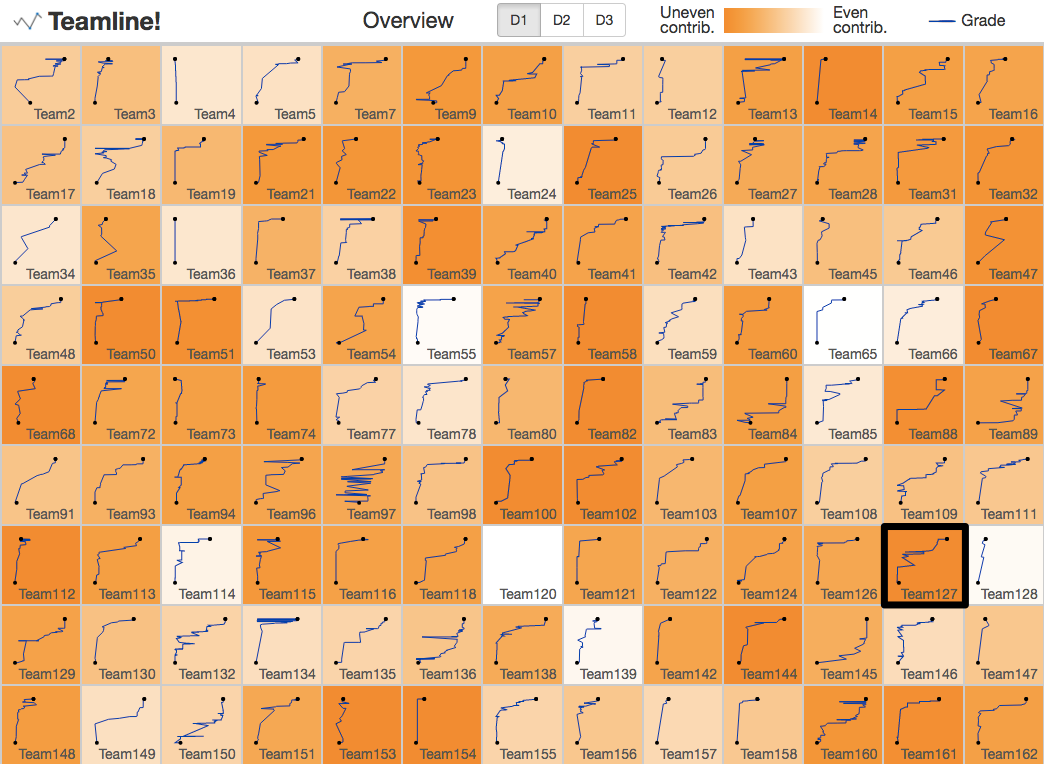
\includegraphics[width=\linewidth]{sample-overview}
  \caption{Sample overview}
  \label{fig:sample-overview}
\end{figure}

\begin{figure}[h]
  \centering
  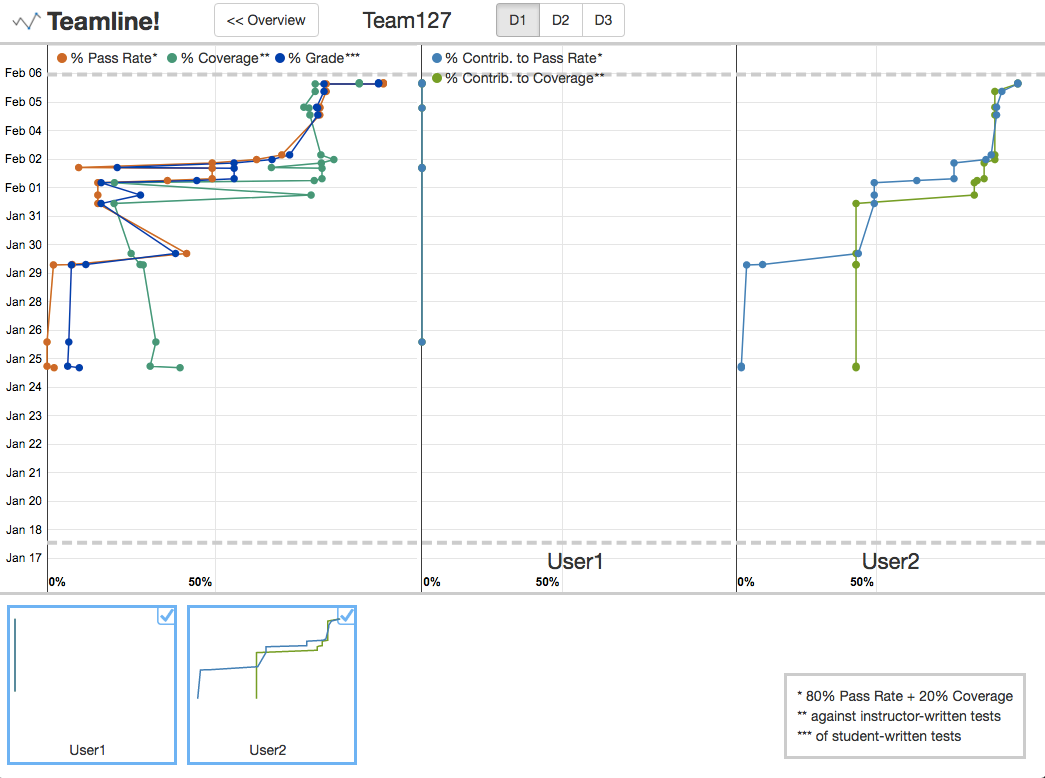
\includegraphics[width=\linewidth]{sample-teamview}
  \caption{Sample team view for Team127}
  \label{fig:sample-teamview}
\end{figure}



% \begin{table}
%   \label{tab:analysis}
%   \caption{What-Why-How analysis of Teamline.}
%   \begin{tabularx}{\columnwidth}{ l | l }
%     \hline
%     What: Data & Table of graded commits. \\
%     What: Derived & \parbox{6cm}{Measure of contribution to pass rate and coverage. Contribution uniformity.}  \\
%     Why: Tasks & \parbox{6cm}{Present the uniformity of contributions and summarize the team's commit history.} \\
%     How: Encode & \parbox{6cm}{We used a heatmap in the overview with}  \\
%     How: Facet & \parbox{6cm}{Overview + detail views. Detail view is partitioned into side-by-side views.} \\
%     How: Embed & \parbox{6cm}{Superimpose sparklines on the overview's heatmap cells.} \\
%     How: Reduce & \parbox{6cm}{Filtering is done by selecting the team and the deliverable in}  \\
%     \hline
%   \end{tabularx}
% \end{table}



% \begin{table}[h!]
%   \centering
%   \caption{Caption for the table.}
%   \label{tab:table1}
%   \begin{tabular}{l|c||r}
%     1 & 2 & 3\\
%     \hline
%     a & b & c\\
%   \end{tabular}
% \end{table}

\end{document}
